\documentclass[12pt,letterpaper,titlepage]{report}
\usepackage{fontspec}
\defaultfontfeatures{Mapping=tex-text}
\usepackage{xunicode}
\usepackage{xltxtra}
\usepackage{enumitem}
\setmainfont{Times New Roman}
\usepackage{amsmath}
\usepackage{amsfonts}
\usepackage{amssymb}
\usepackage{multicol}
\usepackage{paracol}
\usepackage{graphicx}
\graphicspath{{img/}}
\usepackage{karnaugh-map}
\usepackage[margin=0.65in]{geometry}
\author{Jacob Abel}
\title{%
	Homework 8
	\\\large ECE2504 CRN:82729
}

\begin{document}
\maketitle
\begin{raggedright}
\raggedcolumns
\paragraph{Question 1:}
Determine the propagation delay of the following circuits in terms of the gate propagation delays. 
\begin{description}[noitemsep]
\item[$t_{pdNOT}:$] propagation delay of an inverter 
\item[$t_{pdAND}:$]  propagation delay of a 2-input AND gate 
\item[$t_{pdOR}:$] propagation delay of a 2-input OR gate 
\end{description}
Give your answers in a form similar to $5 t_{pdAND} + 2 t_{pdOR} + 3 t_{pdNOT}$  
\begin{multicols}{2}
\begin{enumerate} [label=\alph*)]
\item (2 pts) 4x1 multiplexer (see Figure 3‐25) 
\includegraphics[width=0.4\textwidth,height=0.9\textheight,keepaspectratio=true]{hw8p1a}
\begin{align*}
t_{pd4x1Mux}=& t_{pdNOT}+2t_{pdAND}+t_{pdOR}
\end{align*}

\item (2 pts) Full adder (see Figure 3‐42) 
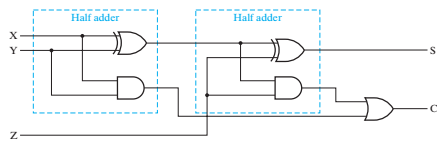
\includegraphics[width=0.4\textwidth,height=0.9\textheight,keepaspectratio=true]{hw8p1b}
\begin{align*}
t_{pdFA}=& t_{pdAND}+t_{pdOR}+t_{pdXOR}
      \\=& t_{pdAND}+t_{pdOR}
      \\+& t_{pdAND}+t_{pdOR}+t_{pdNOT}
      \\=& 2t_{pdAND}+2t_{pdOR}+t_{pdNOT}
\end{align*}

\item (2 pts) 4‐bit ripple carry adder (see Figure 3‐43) 
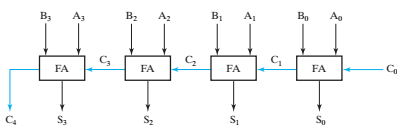
\includegraphics[width=0.4\textwidth,height=0.9\textheight,keepaspectratio=true]{hw8p1c}
\begin{align*}
t_{pdRippleAdder}=& 4t_{pdFA}
               \\=& 4(2t_{pdAND}+2t_{pdOR}+t_{pdNOT})
               \\=& 8t_{pdAND}+8t_{pdOR}+4_{pdNOT}
\end{align*}
\columnbreak

\item (2 pts) the logic circuit shown in Figure 8‐6 
\includegraphics[width=0.35\textwidth,height=0.9\textheight,keepaspectratio=true]{hw8p1d}
\begin{align*}
t_{pd}=& t_{pdXOR}+t_{pd4x1Mux}
    \\=& t_{pdAND}+t_{pdOR}+t_{pdNOT}
    \\+& t_{pdNOT}+2t_{pdAND}+t_{pdOR}
    \\=& 3t_{pdAND}+2t_{pdOR}+2_{pdNOT}
\end{align*}

\item (2 pts) the arithmetic circuit shown in the Case Study 2 Sample Solution
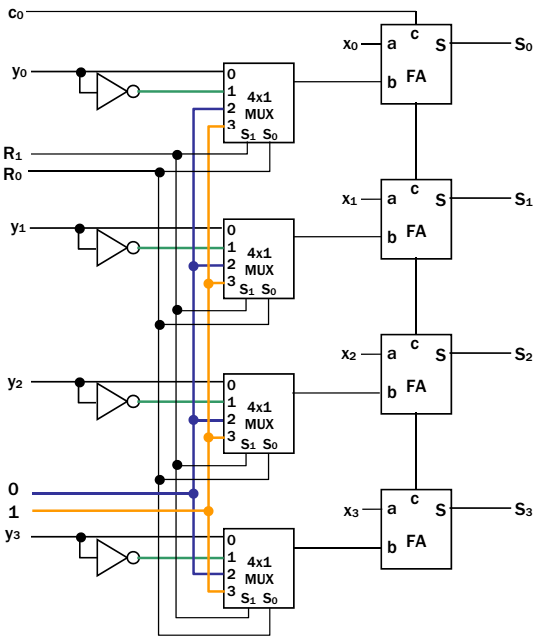
\includegraphics[width=0.35\textwidth,height=0.9\textheight,keepaspectratio=true]{hw8p1e}
\begin{align*}
t_{pd}=& t_{pdXOR}+t_{pd4x1Mux}
    \\=& t_{pdAND}+t_{pdOR}+t_{pdNOT}
    \\+& t_{pdNOT}+2t_{pdAND}+t_{pdOR}
    \\+& 2t_{pdNOT}+3t_{pdAND}+2t_{pdOR}
\end{align*}

\end{enumerate}
\end{multicols}
\clearpage

\paragraph{Question 2:}
(5 pts) Use contraction beginning with a 4‐bit adder to design a 4-bit circuit that subtracts 4 from the 4‐bit input. The function to be implemented is $Z=X-4$. What does contraction mean? Do this:
\begin{itemize}[noitemsep]
\item Recall the Boolean expressions for full adders. $S_i=A_i \oplus B_i \oplus C_i$ and $C_{i+1} = A_iB_i + A_iC_i + B_iC_i$
\item Substitute for the known values in the equations for all four full adders to simplify the expression. For example, if $A=0001, A_3=0, A_2=0, A_1=0, A_0=1,$ which will result in terms such as $A_3B_3$ reducing to 0.
\item Recall the necessary $B$ and $C_0$ inputs to subtract using a 4‐bit adder.
\end{itemize}
\begin{multicols}{3}
\begin{align*}
B=&\overline{0010}=1101\\
C_0=&1
\end{align*}
\begin{align*}
S_0=&(A_0\oplus 1)\oplus 1=A_0
\\C_0=&A_0 1+A_0 1+1(1)=1
\end{align*}
\begin{align*}
S_1=&(A_1\oplus 0)\oplus 1=\overline{A_1}
\\C_1=&A_1 0+A_1 1+0(1)=1
\end{align*}
\begin{align*}
S_2=&(A_2\oplus 1)\oplus 1=A_2
\\C_2=&A_2 1+A_2 1+1(1)=1
\end{align*}
\begin{align*}
S_3=&(A_3\oplus 1)\oplus 1=A_3
\\C_3=&A_3 1+A_3 1+1(1)=1
\end{align*}
\end{multicols}
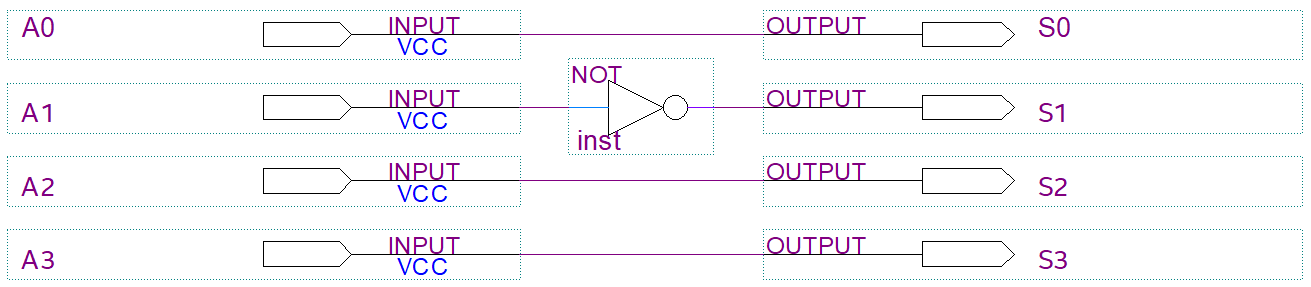
\includegraphics[width=\textwidth,height=0.9\textheight,keepaspectratio=true]{hw8p2}
\clearpage

\paragraph{Question 3:}
(10 pts) Design a combinational circuit that increments its 3‐bit input when $S=0$ and decrements its input when $S=1$. (Note that incrementing means adding 001 and decrementing means subtracting 001 using 2cm arithmetic.)
\begin{enumerate} [label=\alph*)]
\item Design a simplified 2‐level circuit plus inverters as needed for the inputs. (Hint: This means use K maps.)
\begin{paracol}{3}
\begin{karnaugh-map}[2][2][1][$S$][$B_2$]
  \minterms{1,3}
  \autoterms[0]
  \implicant{1}{3}
\end{karnaugh-map}
\centering$B_2=S$
\switchcolumn
\begin{karnaugh-map}[2][2][1][$S$][$B_1$]
  \minterms{1,3}
  \autoterms[0]
  \implicant{1}{3}
\end{karnaugh-map}
\centering$B_1=S$
\switchcolumn
\begin{karnaugh-map}[2][2][1][$S$][$B_0$]
  \minterms{0,1,2,3}
  \autoterms[0]
  \implicant{0}{3}
\end{karnaugh-map}
\centering$B_0=1$
\end{paracol}
\item Start with a 3‐bit ripple carry adder and use a process similar to Case Study 2 to design the circuit.
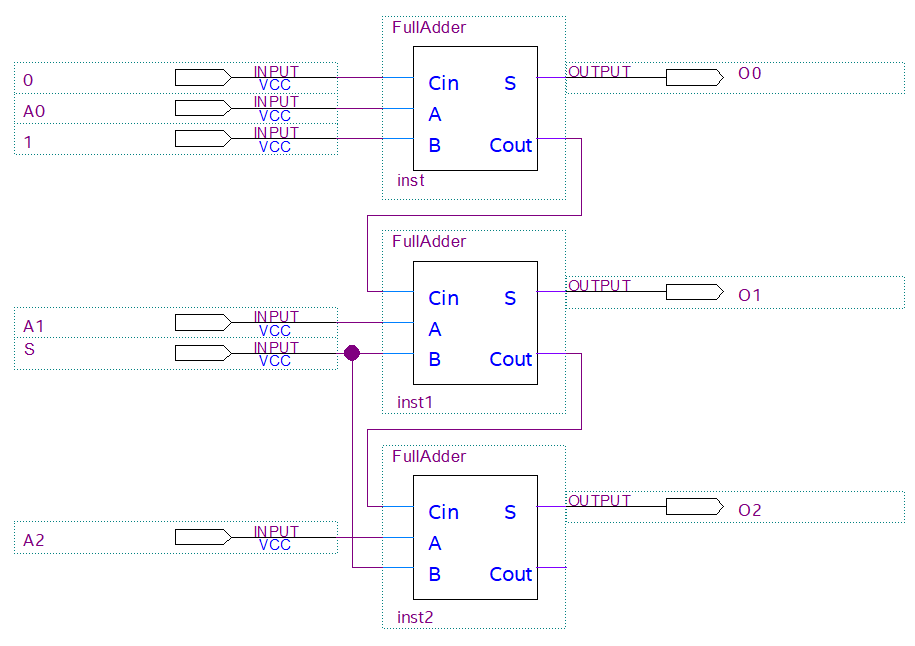
\includegraphics[width=0.9\textwidth,height=0.9\textheight,keepaspectratio=true]{hw8p3}
\item Determine the (2‐input) gate count and propagation delay for parts a and b. Use a form similar to Problem 1
\begin{align*}
t_{pdb}=&3t_{pdFA}
     \\=& 6t_{pdAND}+6t_{pdOR}+3t_{pdNOT}
\end{align*}
\end{enumerate}
\clearpage

\paragraph{Question 4:}
(5 pts) Consider the adder‐subtractor circuit shown in the figure below. For the following inputs, determine the values of the outputs $S_3$, $S_2$, $S_1$, $S_0$, and $C_4$.
\begin{center}
\includegraphics[width=\textwidth,height=0.9\textheight,keepaspectratio=true]{hw8p4}
\end{center}
\begin{center}
\def\arraystretch{1.5} 
\begin{tabular}{cccccc}\hline 
$S$ & $A$ & $B$ & $A +(B\oplus S)$ & $S_3S_2S_1S_0$ & $C_4$ \\\hline 
1 & 1010 & 0111 & 1010+1001 & 0011 & 1 \\ 
0 & 0111 & 0110 & 0111+0110 & 1001 & 0 \\ 
0 & 1010 & 1101 & 1010+1101 & 0111 & 1 \\ 
1 & 1010 & 0011 & 1010+1101 & 0111 & 1 \\ 
1 & 0111 & 1001 & 0111+0111 & 1110 & 0 \\\hline
\end{tabular}
\end{center}

\vspace{\fill}
\noindent
GRADING SCALE
\medskip

Total: 30 pts
\bigskip

\def\arraystretch{1.5} 
\begin{tabular}{ | l | c | c | c | c | c | c | c | c | } \hline
Pts          & 0  & 3  & 7  & 11 & 15 & 18 & 22 & 26     \\\hline
Letter Grade & D- & D  & C- & C  & B- & B  & A- & A      \\\hline
\end{tabular}
\end{raggedright}
\end{document}